\section{Ergebnisse}

\subsection{Gegenseitige Validierung / Intra-DB Validierung}

\cite{intradbvalid}

\subsection{Patienten-DB}

FHIR ConceptMap curl \cite{curl}

\begin{figure}[H]
    \centering
    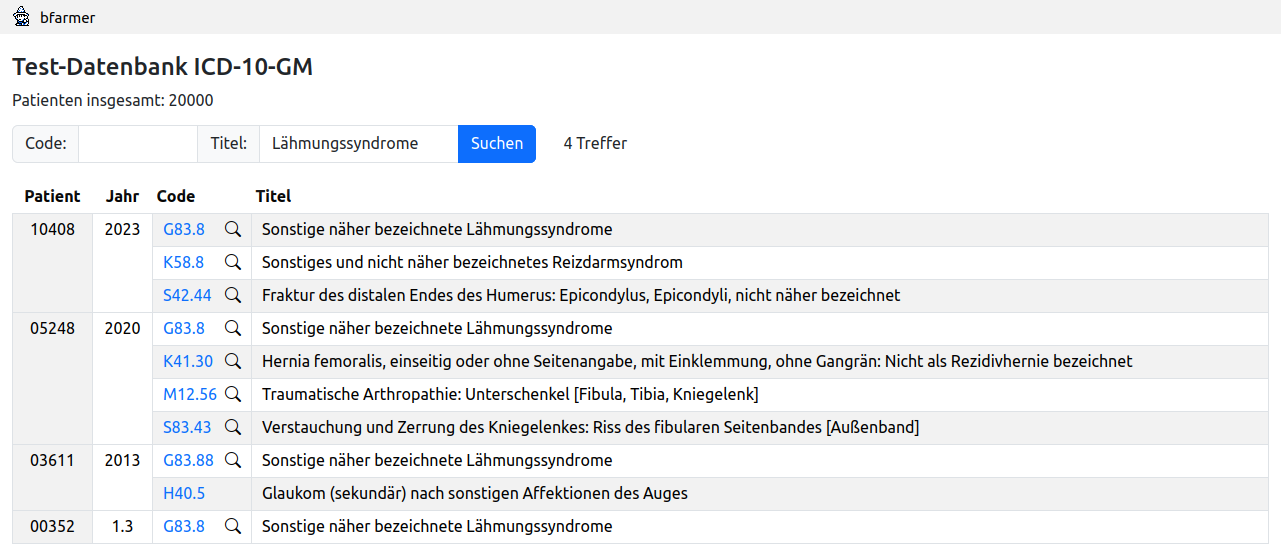
\includegraphics[width=.8\linewidth]{../img/patients_screenshot.png}
    \caption{Patienten}
\end{figure}

\begin{figure}[H]
    \centering
    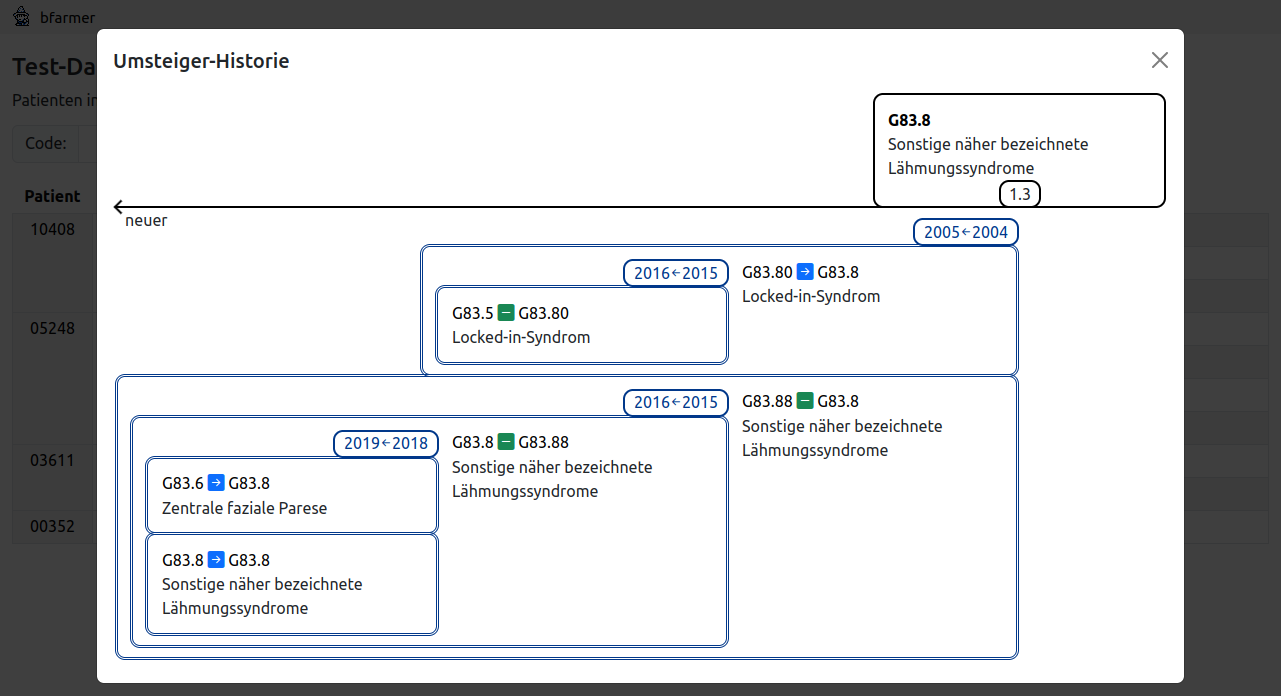
\includegraphics[width=.8\linewidth]{../img/umsteiger_screenshot.png}
    \caption{Umsteiger}
\end{figure}

Integration:

\begin{enumerate}
\item Bootstrap
\item CSS-Datei
\item On-Click Event
\item Ajax-Funktion
\end{enumerate}

\subsection{Mapping Quality}

Beurteilung der generierten ConceptMaps anhand der Qualitätsstandards aus Abschnitt \ref{quali-map}:



\section{Zusammenfassung}

\section{Ausblick}

Folgende Weiterentwicklungen sind sinnvoll.

\subsection{RESTful}

Die Web-Applikation sollte nicht nur teilweise, sondern komplett dem REST-Paradigma entsprechen, wie in Abschnitt \ref{rest-paradigm} aufgeführt. 

Das bedeutet alle Informationen des Servers durch Schnittstellen bereitzustellen: 

\begin{itemize}
\item Kodes als FHIR Code System
\item Umsteiger pro Version im JSON-Format, AJAX für Übersichtseite
\item Ergebnis der horizontalen Suche im JSON-Format
\item ConceptMap ohne Formular
\end{itemize}

Außerdem sollten die Schnittstellen dokumentiert sein über Swagger UI \cite{swagger}.

Bei einem wirklich produktiv eingesetzten System wäre es zudem sinnvoll folgende Dinge zu cachen:

\begin{itemize}
\item Umsteiger-Ergebnisse
\item ConceptMaps
\end{itemize}

Das würde allerdings sehr viel mehr an Speicherplatz benötigen. 

\subsection{ATC}

ATC \cite[ATC-Klassifikation]{bfarmatc}

PDF \cite{poppler}

\subsection{Sessions}

